\cotefile{85}
\scanpage{2}
% L1
\uline{Question} du centre de $\Gamma=G_2/{-}$

\noindent\textcircled{1}\(\left\{\vphantom{\rule{0pt}{30mm}}\right.\)\begin{minipage}{.88\linewidth}
% L2
Représentations \inserted{n. dég.} \deleted{de} $G_0=\mathbb Z_{/2}$

% L3
Représentations \inserted{simplem\unsure{ent}} dégénérées de $\mathbb D_\infty=G_1$ -- i.e. représ. \inserted{fidèles} de $\mathbb D_2$ / relation
% L4
avec oct-aèdre, ou quaternions / quaternions généralisés\ldots.

% L5
Représentations simplement dégénérées de $G_2$ -- i.e.
% L6
représentations n.\ dég. de $\mathbb D_\infty\times\mathbb Z_{/2}$ [\deleted{considérer}\inserted{déterminer}
% L7
les cartes correspondantes, et leur genre\ldots.]

% L8
Représentations doublem\unsure{ent} dégénérées de $G_2$ -- i.e. repr.
% L9
de $\mathbb D_2\times\mathbb Z_{/2}\simeq{\mathbb Z_{/2}}^3$ \deleted{avec} de ``rang'' \deleted{\unsure{égal}} $\geqslant 2$
\end{minipage}

\noindent\rule{.33\linewidth}{.4pt}

% L10
\textcircled{\scriptsize $1'$}\quad$\Vert\!\mid$\quad Pts de ramification des repr. \deleted{de} $G_2$ \ldots

\noindent\rule{.33\linewidth}{.4pt}

% margin note written sideways
\margin{cf verso}
\noindent\(\left\{\vphantom{\rule{0pt}{34mm}}\right.\)\begin{minipage}{.91\linewidth}
% L11
Groupes et cartes associés aux représentations \inserted{projectives}
% L12
de $G_2$ \deleted{dans} un corps -- notamment sur
% L13
un corps fini

\noindent\rule{.60\linewidth}{.4pt}

% L14
Les rev. \deleted{de degré}\inserted{étales modérés} de genre $0$ de la
% L15
sphère privée de trois points

\noindent\rule{.60\linewidth}{.4pt}

% L16
Les cartes finies associées aux hyperpolygônes
% L17
réguliers finis (cf verso)
\end{minipage}

\noindent\rule{.37\linewidth}{.4pt}

\noindent\textcircled{2}\(\left\{\vphantom{\rule{0pt}{16mm}}\right.\)\begin{minipage}{.87\linewidth}
% L18
Terminer de regarder les syst. de \unsure{Schwartz|Schwarz} pythagoriciens
% L19
(cas de $G_5$), et déterminer
% L20
\deleted{\unsure{l'explicitation|l'explication}} la structure de leurs : op. sous les
% L21
gpes des op. élémentaires, dans les trois cas
\end{minipage}

\noindent\rule{.30\linewidth}{.4pt}

\noindent\textcircled{4}\(\left\{\vphantom{\rule{0pt}{10mm}}\right.\)\begin{minipage}{.87\linewidth}
% L22
structure des gpes des op. élémentaires,
% L23
et relations avec $\mathrm{Gal}(\overline{\mathbb Q}/\mathbb Q)$
\end{minipage}

\noindent\rule{.41\linewidth}{.4pt}

% L24
\textcircled{3}\quad Détermination des hyperpolygônes pythagoriciens \unsure{(leurs} \deleted{\unsure{auto}} \unsure{d'équations|l'équation|l'ambiguïté}\unsure{$\{\ldots\}$)}
% archive sheet number: 1
\scanpage{3}
% L1
\deleted{Toute} \unsure{Tout|Toute} \deleted{représentation}\inserted{épi.} du gpe \deleted{\unsure{$L$}}
% L2
\[L_{\deleted{2}3}=\{\rho_0,\rho_1,\rho_2\mid\rho_0\rho_1\rho_2=1\}\]
% L3
dans un gpe fini $\Gamma$ donne une carte finie
% L4
\deleted{homogène} $3$-pondérée homogène (ou régulière,
% L5
ou galoisienne) -- avec l'étude arithmétique
% L6
\unsure{à la} clef. Donc $\forall$ hom de $L_2$ dans un
% L7
$GP(1,k)$, \deleted{donne} à image finie, donne une telle
% L8
carte -- or les représentations en question
% L9
ont une interprétation géométrique
% L10
élémentaire, en termes d'hyperpolygônes
% L11
réguliers. Donc on a une étude
% L12
arithmétique \unsure{directe|de tte} de ceux-ci -- en
% L13
commençant par ceux qui sont
% L14
définis par des systèmes de \unsure{Schwartz|Schwarz}
% L15
\deleted{hyper} pythagoriciens. \unsure{Ceux-ci|Ceux qui} définissent
% L16
44 types de \unsure{'}hyperpolygônes -- \unsure{stables|obtenus} par
% L17
\deleted{symétrie}\inserted{$\unsure{\mathfrak S_3|\mathcal S_3}$} $\times$ ``opérations élémentaires'' --
% L18
et il y a un \deleted{gros}\inserted{(plus petit \unsure{(et fort gros!)|c'est fort gros!} )} quo. \deleted{\unsure{très}} fini de
% L19
$L_2$ qui les coiffe tous.

% L20
\deleted{D'autres exemples sont liés aux}\inserted{Parmi ceux-ci, on a \deleted{ceux} correspondant aux}
% L21
systèmes de Schwartz \uline{canoniques}
% L22
des $n$-gones pythagoriciens de $GP(1)$,
% L23
ou encore, aux bipyramides régulières habituelles
% L24
-- plus leurs transformés par $\mathfrak S_3$.

% margin note written sideways
% L25
\margin{Il convient d'y ajouter ceux qui sont ``dégénérés'', i.e. qui correspondent de trois façons différentes aux représentations de $\mathbb D_\infty\times\mathbb Z_{/2}$, et enfin les hyperdégénérés (représentations \deleted{\unsure{presque}} abéliennes de $G_2$) et \unsure{stabiliser|stabilisés} par $\mathfrak S_3$ et opérations élémentaires\ldots.}
% archive sheet number: 2
\scanpage{4}
% L1
\mspage{(7)}
% L2
Représentations projectives de $G_2$
% L3
(cas non dégénéré i.e.
% L4
non \unsure{diédral|dièdral})
% archive sheet number: 3
\scanpage{5}
% L1
Soient $\Gamma$ un groupe, $(\underline{\tau}_i)_{0\leq i\leq2}$ \deleted{\unsure{un}} syst. de générateurs de $\Gamma$, avec $\underline{\tau}_i^2=1$, $\underline{\tau}_0\underline{\tau}_2=\underline{\tau}_2\underline{\tau}_0$
% L2
On pose $\underline{\rho}_0=\underline{\tau}_0\underline{\tau}_1$, $\underline{\rho}_1=\deleted{\unsure{\tau_2\tau_1}}\;\underline{\tau}_1\underline{\tau}_2$.

% L3
\uline{Thm} \deleted{Soit} $S$ schéma, \deleted{\unsure{$G$ une forme de $GP(1)_S$}, \unsure{$G$ un groupe abstrait}}
% L4
\deleted{\unsure{eng.}} Considérons :

% L5
A) Catégorie $C$ des couples $(G,\varphi)$, où $G$ est une forme de
% L6
$\underline{GP}(1)_S$, $\varphi:\Gamma\longrightarrow G(S)$, satisfaisant les conditions
% L7
$(*)\ \forall s\in S$, $\rho_{0s}^{2}$ et $\rho_{1s}^{2}$ sont $\ne1_s$ [ NB on désigne par $\tau_0,\tau_1,\tau_2,\rho_0,\rho_1$ les
% L8
images de $\underline{\tau}_0,\underline{\tau}_1,\underline{\tau}_2,\underline{\rho}_0,\underline{\rho}_1$ dans $G(S)$ ] et $\rho_{0s}$ et $\rho_{1s}$ ne commutent pas

% L9-13
\deleted{$(\Leftrightarrow)$ b) $\forall s\in S$, l'image $\Gamma_s$ de $\Gamma$ dans $G(s)$ [$\simeq\Gamma/N_s$, où $N_s$ est le noyau de $\Gamma\to G(s)$] \uline{n'est} pas isomorphe à un groupe diédral $\mathbb D_n$ \unsure{($n\geq2$, fini)|($n\geq3$)} $\geq3$ -- le cas $n=1$ ou $2$ est déjà exclu par a), qui signifie que $\tau_{0s}$ et $\tau_{1s}$ ne commutent pas, ni $\tau_{1s}$ et $\tau_{2s}$ -- donc $\Gamma_s$ n'est pas commutatif].}
% L10a
\inserted{\deleted{(ou : un produit $\mathbb D_\infty\times\mathbb Z_{/2}$ \unsure{$\text{ou }\mathbb Z_{/2}\times\mathbb Z_{/2}$})}}
% L11a
\margin{\deleted{On peut remplacer b) par b') $\rho_0$ et $\rho_1$ ne commutent pas (ou encore $\rho_0$ et $\sigma=\rho_0\rho_1=\tau_0\tau_2$ ne comm. pas (NB $\sigma^2=1$)}}

% L14
Les flèches de $C$ sont les isomorphismes.

% L15
B) La catégorie discrète $C'$ définie par l'ens des couples
% L16
$(\deleted{\unsure{\beta_0(\varphi)|\alpha_0(\varphi)}}\alpha_0\unsure{(\varphi)},\deleted{\unsure{\beta_1(\varphi)|\alpha_1(\varphi)}}\alpha_1\unsure{(\varphi)})\in\Gamma(S,\underline O_S)^2$, satisfaisant les conditions
% L17
\[\begin{aligned}&\deleted{\unsure{\beta_0,\beta_1,\beta_0-4,\beta_0+\beta_1}\ \text{sont}}\\
% L18
&\alpha_0+2,\ \alpha_1+\unsure{2|1},\quad\alpha_0+\alpha_1\quad\text{sont inversibles.}\end{aligned}\tag*{(*)}\]

% L19
Pour tout objet \deleted{\unsure{de}} $(G,\varphi)$ de $C$, soit
% L20
\[\alpha_0=A(\deleted{\unsure{\varphi}}\rho_0),\quad\alpha_1=A(\varphi_1)\]
% L21
où
% L21a
\[A:G\mathbin{-}\mathbb E^1_S\]
% L22
est l'invariant. \deleted{On trouve} Ceci posé

% L23
1) $(\alpha_0,\alpha_1)$ ainsi associé à $(G,\varphi)$ satisfait $(*)$

% L24
2) Le foncteur
% L25
\[ C\longrightarrow C' \]
% L26
défini ainsi par $(G,\varphi)\longmapsto(\alpha_0(\varphi),\alpha_1(\varphi))$ est \uline{\unsure{pl\textsuperscript{t}.|pl.} fidèle},
% L27
et c'est une \unsure{$\left.\right\}$} équivalence de catégories \inserted{si $\Gamma=\{\tau_0,\tau_1,\tau_2\mid\tau_0^2=\tau_1^2=\tau_2^2=(\tau_0\tau_2)^2=1\}=G_2$.} En d'autres termes

% L28
a) Le groupoïde $C$ est \uline{rigide}, i.e. $\forall (G,\varphi)$, le centralisateur de
% L29
$\varphi$ dans $G(S)$ est $\{1\}$.

% L30
b) Deux objets $(G,\varphi)$ et $(G',\varphi')$ de $C$ sont isom ssi
% L31
\[\alpha_0(\varphi)=\alpha_0(\varphi'),\quad\alpha_1(\varphi)=\alpha_1(\varphi')\]

% L32
c) \inserted{Si $\deleted{\unsure{G}}\Gamma=G_2$} $\forall$ couple $(\alpha_0,\alpha_1)$ \deleted{\unsure{$\in A$}} de sections de $\underline O_S$ satisfaisant $(*),$
% L33
$\exists\ (G,\varphi)$ \deleted{tel q} $\mathrm{Ob}\ C$ tel que $\alpha_0(\varphi)=\alpha_0$, $\alpha_1=\alpha_1(\varphi)$ [et
% L34
ledit objet de $C$ est défini à isom. unique près grâce à a)]
% archive sheet number: 4
\scanpage{6}
% L1
\uline{Démonstration}\qquad 1) On sait, par les généralités sur les
% L2
polyèdres réguliers, que les conditions a) b) impliquent
% L3
l'existence d'un $2$-polyèdre régulier \inserted{paramétré} épinglé, donnant lieu à
% L4
la repr. $\widehat\varphi:G_2\ (\text{groupe cartographique})\longrightarrow\deleted{\unsure{G}}\Gamma\xrightarrow{\varphi}G(S)$, \deleted{d'où on}
% L5
\deleted{déduit, on l'a vu, que $\alpha_0+2,\alpha_1+2,\alpha_0+\alpha_1$ sont inversibles.}
% L6
défini à isom unique près. Un calcul immédiat
% L7
donne que les invariants $\alpha_0,\alpha_1$ de ce $2$-polyèdre ne sont
% L8
autres que $\alpha_0(\varphi)$ et $\alpha_1(\varphi)$. En effet, dans le contexte général
% L9
(dim $n$) avec paramètres $\beta_i=\alpha_i\unsure{+2|-2}$, on a pour $0\leq i\leq n-1$
% L10
\[ f(a_i)=(\beta_0\cdots\beta_{i-1})\quad f(a_{i+1})=\beta_0\cdots\beta_i\quad \varphi(a_i,a_{i+1})=-(\beta_0\cdots\beta_{\unsure{i|i-1}}) \]
% L11
donc si les $\beta_i$ \deleted{sont inv.} \inserted{ainsi que 2,} on peut \deleted{\unsure{faire}} parler de ``l'angle'' $\theta_i$
% L12
de $a_i$ et $a_{i+1}$, on aura
% L13
\[4\cos^2\theta_i=\frac{\varphi(a_i,a_{i+1})^2}{f(a_i)f(a_{i+1})}=\beta_i\qquad(\underline{\mathrm{NB}}\ \zeta_i=\frac{\beta_i}{\mu_i\mu_{i+1}}=\frac{\beta_i}{4}=\cos^2\theta_i).\]
% L14
\[\text{i.e.}\qquad\alpha_i=2(\underbrace{2\cos^2\theta_i-1}_{\cos2\theta_i})=2\cos2\theta_i\]

% L15
Il faut \unsure{donc prouver|au préalable|aussi prouver} ceci :

% L16
\uline{Lemme} (\deleted{\unsure{si car $\ne2$}}\inserted{si $2$ inv}) Soit $(V,f)$ un module quadratique
% L17
lisse de rang $3$, considérons une rotation \deleted{\unsure{de l'axe}} $\rho$
% L18
d'angle $\deleted{\unsure{\theta_i,\,2\theta_i}}\vartheta$ (autour d'un axe tot\textsuperscript{t} non isotrope)
% L19
et soit $\alpha=2\cos\vartheta$. \deleted{Alors} Soit \deleted{\unsure{$Q$}} $Y\subset\check{\mathbb P}(V)$ fibré
% L20
\deleted{des} droites projectives défini par $f$, et considérons
% L21
l'autom $\rho_Y$ \unsure{induit $\rho$|induit} par $\rho$. Ceci posé, l'invariant
% L22
de $\rho_Y$ est donné par
\figure{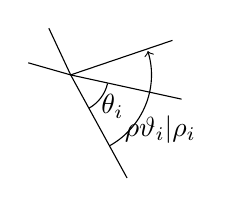
\begin{tikzpicture}[scale=.77]
\draw (-.7,.2)--(0,0)--(1.83,-.40);
\draw (-.36,.77)--(0,0)--(.93,-1.70);
\draw (0,0)--(1.68,.57);
\draw (.30,-.55) arc[start angle=-61,end angle=-13,radius=.63];
\node at (.69,-.52){$\theta_i$};
\draw[->] (.64,-1.17) arc[start angle=-61,end angle=17,radius=1.34];
\node at (1.48,-.90){$\deleted{\unsure{\rho}}\unsure{\vartheta_i|\rho_i}$};
\end{tikzpicture}}
% L23
\[ A(\rho_Y)=\alpha \]

% L24
\uline{Dém} Quitte à choisir des axes de coordonnées convenables
% L25
(possible loc fppf) \deleted{\unsure{SPS}} $f(x,y,z)=x^2+yz$,
% L26
$\rho_{\zeta}(x,y,z)=(x,\deleted{\unsure{\zeta_i}}\zeta y,\zeta^{-1}z)$, et $\alpha=\zeta+\zeta^{-1}$. Or l'hom
% L27
$G_m\hookrightarrow G=\mathrm{Aut}\ C$, $\zeta\unsure{\mathbin{-}|\mapsto}\rho_{\zeta}$, est mono, donc on
% L28
trouve $A(\rho_\zeta)=\zeta+\zeta^{-1}=\alpha$, cqfd.
% archive sheet number: 5
\scanpage{7}
% L1
On a un peu salopé la présentation, \deleted{\unsure{p}} qui suppose
% L2
pour le moins \deleted{\unsure{la}} car. \unsure{rés.} $\ne2$ (sans parler d'une
% L3
``théorie des angles'' sur schéma quelconque, que je
% L4
n'ai pas bien explicitée. Mais il est clair par
% L5
principe du prolongement que si la formule \inserted{sur l'invariant} est
% L6
prouvée en \deleted{car $2$.} $0$ (où on se sent sur terrain
% L7
solide) elle l'est en car. quelconque\ldots

% L8
Comme on est dans le cas de forme \inserted{quad} (\unsure{invariante non|invariante à hom}
% L9
id.\ nulle sur \deleted{\unsure{la}}\inserted{aucune} fibre) lisse, on doit bien avoir
% L10
$(\alpha_0+2)(\alpha_0-2)(\alpha_0+\alpha_1)$ inv. Inversement, si on part
% L11
d'un couple $(\alpha_0,\alpha_1)$ satisfaisant à ces conditions,
% L12
on sait lui associer un polyèdre régulier,
% L13
avec $\unsure{f_V|f_Y|\text{f.q.}}$ lisse, d'où représentation de $G_2$, correspondant
% L14
à ces valeurs. \deleted{On sait que la cat.}
% L15
\deleted{A) est}

% L16
\uline{Corollaire} \deleted{\unsure{Soient}}\unsure{Soit|Soient} $\unsure{\nu_0,\nu_1|v_0,v_1}$ deux entiers $\geq3$ \inserted{ou infinis}, et supposons
% L17
que l'on ait dans $\Gamma$ un syst\textsuperscript{e} complet de
% L18
relations
% L19
\[\tau_0^2=\tau_1^2=\tau_2^2=(\tau_0\tau_2)^2=(\tau_0\tau_1)^{\nu_0}=(\tau_{\unsure{1|0}}\tau_2)^{\nu_1}=1\]
% L20
i.e. $\Gamma=\Gamma_{\nu_0,\nu_1}$.
% slanted
% L20a
\margin{Supposons pour $i=0,1$, que $\nu_i\cdot1_S$ soit inv. sur $S$ \uline{ou} $\nu_i$ premier (impair puisque $\nu_i\geq3$)}
% L21
\deleted{Alors l'image par le fonc. des facteurs \unsure{de $C'$}} Soit \deleted{\unsure{le $G$ la sous}} $C(\nu_0,\nu_1)$
% L22
la sous-catégorie de $C$ formée des
% L23
$(G,\varphi)$ \inserted{($G$ forme de $\underline{GP}(1)_S$, $\varphi:\Gamma\longrightarrow G(S)$ hom)} tels que l'on ait
% L24
\deleted{$\unsure{\mathrm{i})}\quad\rho_0^{\nu_0}=\rho_1^{\nu_1}=1,$ \unsure{i.e., $\rho$}.}

% L25
a) $\forall s\in S$, $\rho_{0s}$ est d'ordre $\nu_0$, $\rho_{1s}$ d'ordre $\nu_1$ \uline{\unsure{exact\textsuperscript{ement}|exactem\textsuperscript{t}|exactement}}

% L26
b) $\forall s\in S$, \inserted{$\rho_0$ et $\rho_1$ ne commutent pas. \unsure{(en principe)}} \deleted{$\Gamma_s$ n'est pas isom. à un $\mathbb D_n$ \unsure{ni|ni à} $\unsure{\mathbb D_\infty}$}
% L27-30
\deleted{$\mathbb D_\infty\times\mathbb Z_{/2}$ [\uline{NB} Il revient au m à d'exiger que $\rho_{0s}$ et $\rho_{1s}$, ou $\rho_{0s}$ et $\sigma_s$, ne commutent pas, \deleted{et} il \uline{suffit} pour cela, compte tenu de a), que l'on ait : on n'a pas $\nu_0$ impair et $\nu_1=2\nu_0$ ou l'inverse]}
% archive sheet number: 6
\scanpage{8}
% L1
Soit $C'(\deleted{\unsure{p_0,p_1}}\unsure{\nu_0,\nu_1|v_0,v_1})$ la cat. discrète définie par les couples
% L2
$(\alpha_0,\alpha_1)$, \deleted{satisfaisant chacun des \unsure{satisfais|satisfait}} avec \deleted{\unsure{les}}
% L3
\[\text{a)}\qquad(\alpha_0+2)(\alpha_1\unsure{+|-}2)(\alpha_0+\alpha_1)\quad\text{inversible}\]
% L4
et chaque $\alpha_i$ satisfaisant les conditions suivantes
% L5
\[\text{b)}\qquad\Psi_{\nu_i}(\alpha_i)=0\qquad i=0,1\]
% L6
\deleted{\unsure{c)}}
% L7-8
\deleted{Supposons enfin que, si l'un des quand l'un des $\nu_i$ est tel que $\nu_i=2p$ (où $p$ nb premier) impair,}
% L9-11
\deleted{c) Si $\nu_i\cdot1_S$ \deleted{est de la forme $2p$ ($p$ nb premier) \unsure{alors on a} $p$} \inserted{$S$ est} \deleted{est inv. sur $S$} est inversible, \uline{ou} de la forme $2p$ ($p$ nb premier), \inserted{avec $2\cdot1_S$ inv. si $p$ impair,} (ou $\nu_i=p$ (nb premier impair)).}
% slanted
% L11a
\margin{\deleted{Condition ne dépendant que de $S$ et $\nu_0,\nu_1$ pas de l'objet particulier choisi.}}
% L12
Alors on a une équivalence de catégories
% L13
\[ C_{(\nu_0,\nu_1)}\longrightarrow C'(\nu_0,\nu_1). \]
\begin{center}\rule{.11\linewidth}{.4pt}\end{center}

% L14
En effet, il faut prouver, \deleted{\unsure{en supposant}}\inserted{si $\Gamma=\unsure{G|g|G_2|\mathcal G}$}, et
% L15
si $(G,\varphi)$ \inserted{$\in\mathrm{Ob}\ C$} et $(\alpha_0,\alpha_1)$ \inserted{$\in\mathrm{Ob}\ C'$} se correspondent, que
% L16
\deleted{A) les conditions a) b) c) sont satisfaites, ssi on}
% L17
l'on a la condition \deleted{a) ci-dessus sur $\rho_0$ et $\rho_1$}
% L18
\[\deleted{\text{ssi}}\quad\rho_i^{\deleted{\unsure{\rho_0}}\nu_i}=1\quad\text{et}\quad\forall s\in S,\quad\rho_{is}\ \text{d'ordre }\nu_i\text{ exactem\unsure{t}}\tag*{(*)}\]
% L19
ssi on a \unsure{'}
% L20
\[\Psi_{\nu_i}(\alpha_i)=0\quad\deleted{\text{et c) concernant }\nu_i}\tag*{(**)}\]

% L21
\margin{\uline{réf}}\deleted{Or il est} Or on sait que \inserted{(pour $\nu_i\geq3$)}, \deleted{suivant que $\nu_i$}
% L22-23
\deleted{est de la forme $2p$ ($p$ premier) ou $p$ ($p$ premier impair), ou ni l'un ni l'autre, que} \inserted{\deleted{premier, ou}} ça s'exprime
% L24
par la condition $\Psi_{\nu_i}(\alpha_i)=0$ sur l'invariant $\alpha_i$
% L25
de $\rho_i$, plus la condition $\nu_i1_S$ inv. si $\nu_i$ non premier
% L26
:
% L27
\deleted{Cas 1\textsuperscript{o}) $2$ inv. sur $S$ si $p$ impair / mais on a}
% L28
\deleted{Cas 2\textsuperscript{o}) aucune condition suppl. \qquad supp. ou $\nu_i$ inv.}
% L29
\deleted{Cas 3\textsuperscript{o}) $\nu_i$ inv. sur $S$ \qquad / ou 1\textsuperscript{o}) supprimé}
% L30
Ce qui prouve l'équivalence.
% archive sheet number: 7
\scanpage{9}
% L1-3
\deleted{\uline{Remarque} Comme $\alpha_i+2$ est inv i.e. $\alpha_{is}\ne-2$ en tt $s$, cela implique qu'en fait, si \deleted{car.} $\unsure{\nu_i|v_i}=2p$ ($p$ premier \inserted{impair \unsure{donc}}), \deleted{Alors il n'y a pas de $C$} \deleted{on peut en prédire, alors que}}
% L4-5
\deleted{\deleted{et si $S$ contient un pt $s$ de $C'(\nu_0,\nu_1)$ est \unsure{in} car $p$, \unsure{alors que|les $\psi$ sont inv.} Alors $C'(\nu_0,\nu_1)$ est \uline{vide}}}
% L6-9
\deleted{On voit \uline{directmt} que dans ce cas $C(\nu_0,\nu_1)$ est \uline{également} vide : en effet, un \deleted{op.} élément de $G_s$ (forme de $GP(1)_{k(s)}$) ne peut jamais être d'ordre $2p$. Donc il \deleted{serait}\inserted{est} \unsure{raisonnable|vraisemblable},}
% L10-12
\deleted{pour assurer que $C(\nu_0,\nu_1)\deleted{\unsure{\longrightarrow}}\simeq C'(\nu_0,\nu_1)$ soient \uline{évt.} non vides, d'exiger que $\nu_i=2p$ \inserted{($p$ pr. impair)} implique $p$ inv. sur $S$, donc en fait $2p=\nu_i$ inv --}
% L13-15
\deleted{c'est à dire qu'on exige que $\nu_i$ est inv. sur $S$ \uline{ou} \deleted{de la forme $p$} \uline{premier} (impair car $\nu_i\geq3$).}

% L16
Exemples avec $\Gamma_{\nu_0,\nu_1}$ \uline{fini}

% L17
A) $\nu_0=3,\nu_1=3,\qquad\Gamma_{\nu_0,\nu_1}\simeq\unsure{\mathfrak S_4|\mathcal S_4}$. On \deleted{trouve que}\inserted{n'a pas de}
% L18
\deleted{la catégorie des repr. de $\mathfrak S_4$ \unsure{en question}}
% L19
restriction à faire sur $S$. On trouve que la
% L20
cat. des couples $(G,\varphi)$, $G$ forme de $GP(1)_S$,
% L21
$\varphi:\mathfrak S_4\longrightarrow G(S)$ tels que $\forall s\in S$, $\rho_{0s}$ et $\rho_{1s}$ soient
% L22
d'ordre $3$ exactement \inserted{et ne commutent pas}, est \deleted{équivalente à la cat}\inserted{vide si \deleted{$2$ n'est}}
% L23
$2$ ($=(-1)(-1)(-1-1)$ au signe près) n'est pas inversible,
% L24
\deleted{alors} et qu'elle est équivalente à la cat. ponctuelle
% L25
dans le cas contraire. C'est à dire : Si

% L26
a) \deleted{En}\inserted{Sur un corps de} car. $2$, toute une repr. $\mathfrak S_4\unsure{\mathbin{-}|\to}G(S)$, les
% L27
\inserted{$\rho_0$ et $\rho_1$ commutent i.e.} \deleted{$\rho_0$ et $\rho_1$ ou $\rho_1=1$} \deleted{\unsure{i.e. si $\rho_0$ et $\rho_1$ commutent|$\rho_0$ et $\rho_1$ commutent}} \deleted{i.e. $\tau_0\deleted{\unsure{\pm|=}}\tau_1$ ou $\tau_1=\tau_2$ alors} la
% L28
repr. se factorise par $\deleted{\mathfrak S_3(=\mathbb D_3)}\ \deleted{\unsure{\mathfrak S_3}}\ \mathfrak S_3\deleted{\unsure{=\mathbb D_3\subset\mathfrak S_4}}$
% slanted
% L27a
\margin{\deleted{faux?}\ $\big|$}
% archive sheet number: 8
\scanpage{10}
% L1
b) Sur un \deleted{corps de car. $\unsure{=|\ne}$}\inserted{schéma $S$, où $2$ est inv.} (i.e. sur $\mathbb Z[{}^1\!/_2]$), il
% L2
y a à isom unique près, un couple $(G,\varphi)$
% L3
et un seul, où $G$ est une forme de $GP(1)_S$,
% L4
$\varphi:\unsure{\mathfrak S_4|\mathcal S_4}\longrightarrow G(S)$, avec $\rho_{0s}$ et $\rho_{1s}$ \deleted{d'ordre $3$ exactement}\inserted{non commutants}
% L5
en chaque fibre. \inserted{i.e. la repr. ne se factorise par $\mathfrak S_3$ sur aucune fibre} [En fait, \deleted{\unsure{on}} on trouve que
% L6
ladite représentation \deleted{est} \unsure{question|en question|partout} est fidèle]

% L7
B) $\unsure{\nu_0|v_0}=4,\nu_1=3$ (ou l'inverse) -- \deleted{on doit encore supp}\inserted{ici on sait que}
% L8
$\Gamma=\mathfrak S_4\times\mathbb Z_{/2}$. Le résultat général nous dit que
% L9
c'est \inserted{encore} la car. $2$ qu'il faut écarter. [On pourrait
% L10
déduire un énoncé concernant le gpe $\Gamma$ de
% L11
A), mais on préfère le traiter directement, on
% L12
trouve des renseignements suppl.) Maintenant $\underline{\tau}_0,\underline{\tau}_1,\underline{\tau}_2$
% slanted
% L12a
\margin{pas \uline{vraiment}!}
% L13
sont \deleted{d'autres}\inserted{les} \uline{gén. octaédraux} (non plus
% L14
tétraédraux) \unsure{satisfont|satisfaisant|tels que} $\rho_0^4=\rho_1^3=1$, et on
% L15
trouve

% L16
a) Sur un corps de car $2$, $\deleted{\unsure{\exists|\forall}}\forall$ hom \inserted{$\varphi:\Gamma\to G$} de
% L17
$\Gamma\simeq\mathbb Z_{/2}\times\mathfrak S_4$ dans une forme de $GP(1)_k$,
% L18-19
\deleted{\unsure{on a} $\rho_0^2=1$ ou l'ordre de $\rho_0$ est égal à $2$ ou celui $\rho_1=\mathrm{id}$}
% L19a
\inserted{ou $\rho_0$ et $\rho_1$ commutent}
% L20-22
\deleted{(i.e. : ou bien $\tau_0$ et $\tau_1$ commutent \deleted{\unsure{donc}} donc $\tau_2$ : elle se factorise par $\mathbb Z_{/2}\times\mathfrak S_3$, ou bien $\tau_1=\tau_2$ \deleted{\unsure{et}} et elle se factorise par $\mathbb Z_{/2}\times\deleted{\unsure{\mathfrak S_4}}\mathbb Z_{/2}$}
% slanted
% L22a
\inserted{i.e. elle se factorise par $\mathbb Z_{/2}\times\mathfrak S_3\simeq\mathbb D_6$}

% L23
b) Sur un schéma $S$ où $2\,1_S$ est inv,
% L24
$\exists!$ à isom unique près couple $(G,\varphi)$, avec
% L25
$\varphi:\Gamma\longrightarrow G$ forme de $GP(1)$ \inserted{tels que $\varphi_s$ ne se fac pas par $\mathbb Z_{/2}\times\mathfrak S_3\simeq\mathbb D_6$} -- et en fait
% L26
$\varphi$ est trivial sur $\mathbb Z_{/2}=\mathfrak z(\Gamma)$, et induit un
% L27
mono $\mathfrak S_4\subset G_{\unsure{\varphi|s}}(S)\qquad\forall s\in S$.
% archive sheet number: 9
\scanpage{11}
% L1
C) $\unsure{\nu_0|v_0}=3,\nu_1=5,\quad\Gamma_{\nu_0,\nu_1}=\mathbb Z_{/2}\mathbb Z\times\deleted{\unsure{\mathfrak S}}\mathfrak A_5$. On a
% L2
$\alpha_0=-1,\ \alpha_1\inserted{=\alpha}$ \deleted{\unsure{sol}}solution de $\alpha^2+\alpha-1=0$, donc
% L3
$\deleted{\alpha_0+\alpha_1}\quad\alpha_0+2=1,\quad\alpha_1+2\inserted{=\alpha+2}$ inversible ($N(\alpha+2)=-1-2+4=1$,
% L4
$1/(\alpha+2)=\alpha'+2=-\alpha+1$) $\alpha_0+\alpha_1=\alpha-1$ inversible
% L5
($N(\alpha-1)=-1+1+1=1$, $1/(\alpha-1)=\alpha'-1=-\alpha-2$ ] Donc

% L6
\uline{Thm} Pour tt \deleted{hom} couple $(G,\varphi)$, $G$ forme de
% L7
$GP(1)_S$, $\varphi$ hom $\Gamma=\mathbb Z_{/2}\times\mathfrak A_5\longrightarrow G$, soit
% L8
$\alpha(\varphi)$ l'inv. de $\varphi(\rho_1)$. On trouve ainsi une
% L9
équivalence entre la cat. des $(G,\varphi)$
% L10
tels que $\forall s\in S$, \deleted{$\rho_{0s}$ et $\rho_{1s}$ soient d'ordres}\inserted{$\varphi_s\mid\mathfrak A_5$ ne soit pas trivial},
% L11
\deleted{$3$ et $5$ resp et $\rho_0$ et $\rho_1$ ne commutent pas,}
% slanted
% L11a
\margin{Laisser tomber $\mathbb Z_{/2}$ dans l'énoncé [celui sur $\mathbb Z_{/2}$, ou tt \deleted{\unsure{$\leftrightarrow$|$\Leftrightarrow$}} autre \deleted{\unsure{facteur}}\deleted{\unsure{non}} facteur, est un corollaire.]}
% L12
avec la \deleted{\unsure{ens}} cat. discrète \deleted{formée des}
% L13
définie par l'ens des $\alpha\in\Gamma(S,\unsure{\mathcal O_S|\mathscr O_S|\underline{\mathcal O}_S})$ satisfaisant
% L14
l'équation
% L15
\[\alpha^2+\alpha-1=0\]

% L16
Les représentations $\varphi$ sont triviales sur $\mathbb Z_{/2}$,
% L17
donc correspondent \unsure{aussi|ainsi} aux
% L18
$\varphi^+:\mathfrak A_5\longrightarrow G$ qui sont triviales sur
% L19
aucune fibre.
% archive sheet number: 10
\scanpage{12}
% L1
(10 p)
% L2
Représentations projectives
% L3
de $G_1$ (et repr. \deleted{\illegible{1}}
% L4
projectives dégénérées
% L5
de $G_2$)
% archive sheet number: 11
\scanpage{13}
% L1
\deleted{\uline{Lemme}}\inserted{\uline{Prop}} Soit $G$ \inserted{$=\underline{\mathrm{Aut}}(Y)$ ($Y$ droite projective)} forme de $GP(1)$ sur corps $k$ \inserted{alg. clos}, $\tau_0,\tau_1,\tau_2\in G(k)$
% L2
tels que $\tau_0^2=\tau_1^2=\tau_2^2=(\tau_0\tau_2)^2=1$. Conditions équivalentes

% L3
A) $\exists$ \deleted{diviseur} diviseur de degré $2$ sur $Y$ \deleted{tel que}\inserted{stable} par les $\tau_i$

% L4
\leavevmode\llap{\smash{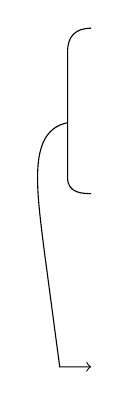
\begin{tikzpicture}[baseline=0pt,x=1mm,y=1mm]
\draw (0,2) .. controls (-2,2) and (-3,1) .. (-3,-1) -- (-3,-17) .. controls (-3,-19) and (-1,-19) .. (0,-19);
\draw[->] (-3,-10) .. controls (-8,-11) and (-7,-18) .. (-6,-26) -- (-4,-41) -- (0,-41);
\end{tikzpicture}}\hspace{1mm}}B) On peut trouver un sous groupe \deleted{alg\unsure{éb}} $H$ de $G$ qui est
% L5
soit \quad a) un $N(T)$, $T$ tore maximal
% L6
\hphantom{soit}\quad b) un $B$, sg groupe de Borel
% L7
tel que les $\tau_i\in H$

% L8
A') Les \deleted{repr. project.} prolongem\unsure{ts} \deleted{projectifs} \inserted{$\tau'_i$ au plan projectif enveloppe $C$} \deleted{\unsure{$\varphi$}} $(i=0,1,2)$
% L9
des $\tau_i$ laissent une droite invariante ($\Leftrightarrow$ si
% L10
car. est $\ne2$ : laissent un pt invariant)

% L11-13
\deleted{C) L'image de \deleted{\unsure{la|des}} $G_2^+$ dans $G(k)$ [i.e. le gpe engendré par $\rho_0=\tau_0\tau_1$ et $\rho_1=\tau_1\tau_2$, ou par $\rho_0$ et $\sigma=\tau_0\tau_{2}=\rho_0\rho_1$] est commutatif}
% L11a
\margin{C''') $\varphi$ se factorise par un groupe $\Gamma'$ ext. \deleted{centrale d'un}\inserted{d'un gpe comm.} \deleted{ce gpe :} par un groupe \uline{cyclique}}
% L13a
\margin{C') $\varphi:G_2\unsure{\mathbin{-}|\to}G(k)$ se factorise à travers un $\mathbb D_\infty\times\mathbb Z_{/2}$}

% L14
\deleted{\unsure{B|C}}\uline{C}) Deux parmi les trois couples $(\tau_0,\tau_1)$ $(\tau_1,\tau_2)$
% L15
$(\rho_0,\rho_1)$ commutent, i.e. ou $\rho_0^2=1$ ou $\rho_1^2=1$ ou $\rho_0\rho_1=\rho_1\rho_0$

% L16
\uline{D}) Le \deleted{\unsure{noyau dans un des op.}}\inserted{ss-groupe de $G(k)$} engendré par les $\tau_i$ est
% L17
isom à un $\mathbb D_n$ ($n\geq1\unsure{\}},$ y c. infini) ou $\mathbb D_{\unsure{n|m|\infty}}\times\mathbb Z_{/2}$ ($n$ pair)
% margin note written sideways
% L17a
\margin{\uline{NB} dans (D), si car $k\ne2$, on peut remplacer les $\mathbb D_n\times\mathbb Z_{/2}$ par $\mathbb D_\infty\times\mathbb Z_{/2}$}

% L18
$A\Leftrightarrow A'$ $\deleted{\Leftrightarrow}$ : traduction via dictionnaire entre $Y$ et $C$ (div. de degré
% L19
$2$ sur $Y\longleftrightarrow\text{droites de }C$)

% L20
$A\Longleftrightarrow B$ car les stabilisateurs des div de degré $2$ sur $Y$
% L21
sont les ss-gpes explicités dans B

% L22
On utilisera que les groupes $H(k)$ sont des produits
% L23
$1/2$-directs $\unsure{\gamma|\mathcal T}.U$, $U$ comm, $\gamma$ \deleted{\unsure{d'un gpe}}\inserted{comm.},
% L24
$ {}_2\gamma$ d'ordre $1$ ou $2$, \unsure{$1/2$ entier|$1/2$ enfin} $ {}_2U$ dans le centre de \deleted{\unsure{de $H$}},
% L25
\deleted{\unsure{et pour voir que}}\inserted{$i_{\varepsilon}$ est l'identité sur $ {}_2U$}. $({}_2\gamma).U$ \unsure{lire|i.e.} $ {}_2\gamma=\{1\}$ ou $ {}_2\gamma=(1,\varepsilon)$, avec \unsure{$\varepsilon\ \mathrm{int}\ \varepsilon\mid H$}.

% L26
$B\Longrightarrow C$ \qquad En effet, \deleted{comme alors} les images des $\tau_i$ dans
% L27
$\gamma$ étant dans $ {}_2\gamma$ \deleted{sont égales} si $ {}_2\gamma=\{1\}$, \deleted{\unsure{que}}\inserted{cas $H=B$},
% L28
en car. $2$) alors l'image $\Gamma'$ de $\Gamma$ dans $G(\unsure{s|k|S})$
% L29
est $\subset H(k)$ donc est comm, on a C.
% L30
Sinon, soit $\gamma=\{1,\varepsilon\}$. Si \deleted{$(\tau_0,\tau_1)$ et $(\tau_1,\tau_0)$}
% L31-32
\deleted{$\tau_0$ et $\tau_1$, $\tau_2$ \unsure{ts} égaux à $1$, c'est comme dessus. Si $\tau_1\,\tau_0$ ne commutent pas, on voit que \unsure{$\tau_2$}}
% L33
on avait $\tau_i\in H(k)$, comme $\tau_i^2=1$, on
% archive sheet number: 12
\scanpage{14}
% L1
conclurait que $\tau_i$ est dans le centre -- ce qui
% L2
n'est pas le cas pour \inserted{ni pour} $i=0$ ni $1$ \deleted{\unsure{ou}} $2$, si $(\tau_0,\tau_1)$ et
% L3
$(\tau_1,\tau_2)$ ne commutent pas. Dans ce cas, on a
% L4
donc $\dot\tau_0,\dot\tau_1,\dot\tau_2$ sont égaux à l'unique élément $\ne1$
% L5
dans $\unsure{\gamma|\mathcal T}$, donc $\rho_0$ et $\rho_1$ sont dans $H$, donc
% L6
commutent. \unsure{$=$}

% L7
$C\Rightarrow\deleted{\unsure{D|A}}C'$) C implique que le \deleted{image} gpe engendré
% L8
par les $\tau_i$ est isom à un quotient d'un
% L9
des trois gpes déduits de $G_2$ en
% L10
divisant par l'une des relations $\deleted{(\tau_0\tau_1)^2=1}$ $\rho_0^2=1$
% L11
$\deleted{\tau_1\tau_2}\ \underline{\rho}_1^{\deleted{\unsure{0}}2}=1$ ou $\underline{\rho}_0\underline{\rho}_1=\rho_1\rho_0$. On voit \unsure{tt|tout} de
% L12
suite que chacun de ces groupes est
% L13
isomorphe à $\Gamma'=\mathbb Z_{/2}\times\mathbb D_\infty$,

% L13a
$C'\Rightarrow C''$\quad \deleted{\unsure{Il suffit que} \unsure{de}}\inserted{\unsure{qui contient}}
% L14
\deleted{un tel groupe, on a} un ss groupe invariant abélien \inserted{cyclique} $\mathbb D_\infty^+=\Gamma''\subset\Gamma'$, 
% L15
à quotient abélien

% L16
$C'')\Rightarrow A)$ Si $u$ est un gén\unsure{,} de $\Gamma''$, et si $u_{\unsure{Y|\gamma|\varphi}}=\mathrm{id}$, l'hom
% L17
se factorise par le gpe comm. \uline{quotient}, et on
% L18
gagne (....). Sinon, le diviseur des pts fixes de
% L18a
\margin{\uline{réf?}}
% L19
$u_Y$ est intrinsèquemt attaché \inserted{\unsure{donc|sous}} au \deleted{\unsure{$q$}} gpe des $\unsure{\mathrm{Aut}_k(Y)|\mathrm{Aut}_Y(k)|\mathrm{Aut}(X)}$
% L20
engendré par $u_Y$, donc stable par $\Gamma'$, on gagne.

% L21
Donc A) à C'') sont équivalents, d'ailleurs
% L22
$D\Rightarrow C'')$, montrons que B) \& C') implique
% L23
D.... Il suffit de prouver que tt ss-gpe d'
% L24
\deleted{$B$ ou $N(T)$} d'un $H=B$ ou $N(T)$ qui est $\inserted{\simeq}$ un
% L25
quotient de $\mathbb D_\infty\times\mathbb Z_{/2}$, est isom. à $\mathbb D_\infty\times\mathbb Z_{\unsure{2|/2}}$ ou
% L26
ou à un $\mathbb D_n$, ou à un $\mathbb D_n\times\mathbb Z_2$.
% archive sheet number: 13
\scanpage{15}
% L1
\uline{Lemme 1} Soit $\mathbb D_\infty=\deleted{\unsure{\mathbb Z_\infty}}\inserted{\{\sigma_0,\sigma_1\mid\sigma_0^2=\sigma_1^2=1\}}$ gpe diédral infini, \inserted{$u=\sigma_0\sigma_1$} \deleted{alors les ss-gpes}
% L2
\deleted{$N$ de $\mathbb D_\infty$, \inserted{\unsure{abél.,}}\inserted{\unsure{et cycl.}} sont les suivants} \deleted{Considérons}

% L2a
a) Soit $i\in\mathbb N^{\deleted{\unsure{*}}}$ (entier $\geq0$) \deleted{\unsure{fini}}
% L3
\deleted{soit $N_i$ le ss-groupe $N_i$ $\forall i\in\overline{\mathbb N}^{*}$, soit} $N_i$ le sous-gpe engendré
% L4
par $u^i$ \deleted{\unsure{($i$ fini), resp. si $i=\infty$)}}. C'est un ss-gpe invariant, \inserted{cyclique infini ($i\ne0$) ou $1$,} de quotient $\deleted{\unsure{\mathbb D_\infty/}}N_i$
% L5
isomorphe à $\mathbb D_i=\{\sigma_0,\sigma_1\mid\sigma_0^2=\sigma_1^2=(\sigma_0\sigma_1)^i=1\}$ (\uline{NB} par déf. $\mathbb D_0=\mathbb D_\infty$)

% L6
b) \deleted{$\forall i\in\overline{\mathbb N}^{\unsure{*}}$, soit $N'_i$}\deleted{le sous-gpe $N'_i$ de $\mathbb D_\infty$ engendré par $u^i$, et}
% L7
Soit $i\in\mathbb N^{\deleted{\unsure{*}}}$, et soit $j\in\mathbb Z/i\,\mathbb Z$. \deleted{Considérons}
% L8
enfin, soit $\deleted{\unsure{H}}N_{ij}$ le sous-gpe de $\mathbb D_\infty$ engendré par
% L9
$u^i$ et $\sigma_0u^{j'}$, avec $j'\in\mathbb Z$, ($j'$ mod $i$) $=j$. C'est un sous-groupe
% L10
\inserted{isom. à $\mathbb D_\infty$ ($i\ne0$) ou $\mathbb Z/2\,\mathbb Z$ ($i=0$),} invariant ssi $\mathbb D_i$ est commutatif i.e. $i\in\{1,2\}$ \deleted{auquel}
% L11
\deleted{cas le} \deleted{Ce gpe contient un conjugué de $\sigma_0$ sss $j\in2\,\mathbb Z/i\mathbb Z$}
% L12
\deleted{(p. ex. si $i$ impair), un conjugué de $\sigma_1$}
% L13
[de plus, si $i$ \deleted{\unsure{inv|est pair}}\inserted{impair}, ce gpe contient des conjugués de $\sigma_0$ et $\sigma_1$ (\deleted{qui sont} car les images sont conjugués)]. --
% L14
\deleted{Il contient un} Quel que soit $i$, $N_{ij}$ contient un conjugué
% L15
de $\sigma_0$ sss $j\in2\,\mathbb Z/i\mathbb Z$, un conjugué de $\sigma_1$ sss $(j+1)\in2\,\mathbb Z/i\mathbb Z$

% L16
c) Les ss-groupes $\{N_i,N_{ij}\}$ sont deux à deux distincts
% L17
et tt sous-gpe de $\mathbb D_\infty$ est l'un de ceux-ci.

% L18
\uline{P. ex} $\{1\}=N_0,\quad\mathbb D_\infty=N_{1,0}$

% L19
\uline{Cor} 1 Les \inserted{types d'iso. des} gpes quotients de $\mathbb D_\infty$ sont \deleted{les}\inserted{ceux} $\mathbb D_i$ ($i\geq1$, $i$
% L20
fini ou infini), \deleted{\unsure{$+$}} et \deleted{\unsure{$\mathbb Z_2$}} du gpe unité.

% L21
\uline{Corollaire} 2 Les \deleted{s-groupes \unsure{$N$} de $\mathbb D_\infty\times\mathbb Z_{/2}$ en}\inserted{\deleted{groupes} types d'iso des gpes quotients}
% L22
de $\mathbb D_\infty\times\mathbb Z_{/2}$ \unsure{ou|sont} les $\mathbb D_i\times\mathbb Z_{/2}$ \inserted{($i$ fini \deleted{\unsure{pair}} ou infini)} et les \inserted{$\mathbb D_i$.}
% L23-26
\deleted{contenus ds le facteur $\mathbb D_\infty$ sont correspondent 1-1 aux couples $N'\subset N''$ de deux ss-gpes de $\mathbb D_\infty$ ($N'=M\cap\mathbb D_\infty$, $N^{\unsure{''|'}}=\mathrm{Im}(M\xrightarrow{\mathrm{proj.}}\mathbb D_\infty)$) \unsure{$\}_2$} \deleted{$\unsure{M}$} de gpe \unsure{$M$} est invariant sss $N,N'$ le sont, ce qui donne}
% margin note at left of the cancelled block
% L24a
\margin{\uline{NB} $\mathbb D_i\times\mathbb Z_{/2}\simeq\mathbb D_{2i}$ si $i$ impair}
% L27
\deleted{Ce sont} \uline{Dém} Ce sont évidemment là des quotients de
% L28
$\mathbb D_\infty\times\mathbb Z_{/2}$ (par $N_i$ resp $N_i\times\mathbb Z_{/2}$). Si $\Gamma=(\mathbb D_\infty\times\mathbb Z_{/2})/N$
% L29
est un gpe quot, où $N$ ss-gpe inv., si $N\subset\mathbb D_\infty$
% L30
$\Gamma\simeq\mathbb D_\infty/N\times\mathbb Z_{/2}$ et on applique cor. 1, sinon $N\xrightarrow{\text{épi}}\mathbb Z_{/2}$
% archive sheet number: 14
